\section{Sharper constants and the price of readout}
\label{sec:sharp-constants}
A uniform exponent is useful, but it does not substitute for a finite-cost
comparison. We now sharpen the constants analytically, keep the cost of
readout visible, and identify which guarantees survive incomplete calibration.

\subsection{A sharper local information and cost envelope}
\begin{lemma}[Sharper pointwise constants]\label{lem:sharp-local}
For every allowed depth and positive noise, write $s=s_t$, $G=G_t$,
$\eta=\eta_t$, and $j=1-\sqrt{1-s^2}$. Then
\begin{equation}\label{eq:sharp-local}
 \frac25s^2G\leq d_M(t)\leq3s^2G.
\end{equation}
For $B=\log(1/\delta)$ and $0<\delta\leq1/4$, the better of the
two counting protocols obeys
\begin{equation}\label{eq:sharp-local-upper}
 \min\{U_Y(t,\delta),U_E(t,\delta)\}
 \leq\frac{9c(t)}{4s^2}\left(1+\frac B G\right).
\end{equation}
\end{lemma}
\begin{proof}
The earlier constructive lower bounds give
$d_M\geq s^2\max\{2,\tfrac12\log(1+\eta)\}$.
For $x\geq0$, $\max\{2,x/2\}\geq(2/5)(1+x)$, proving the lower side.
For the upper side, the fidelity--ratio inequality gives
\[
 d_M\leq4[1+\operatorname{arsinh}\sqrt\eta]j.
\]
The function $\operatorname{arsinh}\sqrt\eta-\log(1+\eta)$ has its
maximum at $\eta=1/3$, with value $\log(3\sqrt3/4)$.
Consequently, with $q_0=1+1/\sqrt2$,
\[
 d_M\leq
 \frac{4[1+\log(3\sqrt3/4)]}{q_0}\,s^2G<3s^2G,
\]
where $j=s^2/(1+\sqrt{1-s^2})\leq s^2/q_0$.

If $\eta<1$, the fixed-$Y$ estimate in the proof of
Proposition~\ref{prop:conclusive-counting} is at most
$(c/s^2)(1+B/G)$. If $\eta\geq1$, then
$\ell_E\geq\log(1+4\eta)$ and
\[
 1+\log(1+\eta)\leq\frac98\log(1+4\eta)\leq\frac98\ell_E.
\]
For the first inequality, the difference of the right and left sides is
positive at $\eta=1$ and has positive derivative thereafter.
Using $b_E\leq1+B/\ell_E$ and $r(1+\cos\vartheta)\leq2$ gives
$U_E\leq(2c/s^2)[1+9B/(8G)]$, which implies the stated bound.
\end{proof}

\begin{theorem}[A factor-27 cost bracket at a fixed depth]
\label{thm:fixed-depth-sharp}
Let $C_{M,\delta}^\star(t)$ restrict every block to depth $t$, while
allowing adaptive POVMs. Under the same positive-noise assumptions,
\begin{equation}\label{eq:fixed-depth-sharp}
 \frac{c(t)}{12s_t^2}\left(1+\frac{\log(1/\delta)}{G_t}\right)
 \leq C_{M,\delta}^\star(t)
 \leq\frac{9c(t)}{4s_t^2}
             \left(1+\frac{\log(1/\delta)}{G_t}\right).
\end{equation}
The upper bound is an attainable stopping cost, and the lower bound
allows all single-block readouts at that fixed depth.
\end{theorem}
\begin{proof}
The affinity and KL converses give
$C^\star(t)\geq c(t)\max\{h_\delta/j_t,k_\delta/d_M(t)\}$.
Put
\[
 h_0=1-\sqrt3/2,\qquad
 \kappa_0=\frac{\log3}{2\log4},\qquad q_0=1+1/\sqrt2.
\]
For $\delta\leq1/4$, $h_\delta\geq h_0$ and
$k_\delta\geq\kappa_0B$: indeed
$k_\delta\geq[B+\log(3/4)]/2$ and $B\geq\log4$.
Thus the lower bound is at least
\[
 \frac c{s^2}\max\left\{h_0q_0,\frac{\kappa_0}{3}\frac B G\right\}.
\]
For $a,b,x>0$, $\max\{a,bx\}\geq ab(1+x)/(a+b)$.
Here $ab/(a+b)>1/12$; the exact expression is
$h_0q_0\kappa_0/(3h_0q_0+\kappa_0)\approx0.0837274$.
Lemma~\ref{lem:sharp-local} supplies the upper bound.
\end{proof}

The factor 27 refers to this fixed-depth envelope. Minimizing its lower
side over depths would not by itself lower-bound a protocol that changes
depth adaptively. The following argument supplies that separate step.

\subsection{A smaller global constant gap}
\begin{theorem}[Explicit constants for adaptive depth]
\label{thm:sharp-global}
In Theorem~\ref{thm:uniform-cost}, let
$S_\delta=A_{\rm eff}[1+\log(1/\delta)/G_{\rm eff}]$. Then
\begin{equation}\label{eq:sharp-global}
 \frac1{70}S_\delta\leq C_{M,\delta}^\star\leq42S_\delta.
\end{equation}
The positive-noise upper bound is attained by choosing
\begin{equation}\label{eq:sharp-depth}
 t_\sharp=\min\{\overline D,\lceil\reff/2\rceil\}
\end{equation}
and then $Y$ counting if $\eta_{t_\sharp}<1$, or conclusive counting
otherwise. The zero-noise convention in Theorem~\ref{thm:uniform-cost}
also satisfies these constants, including at zero error.
\end{theorem}
\begin{proof}
Write $R=\reff$, $x=\mu^2R/\gamma$, $G=1+\log(1+x)$, and
$A=c(R)/(\mu^2R^2)$. For $t\leq R$,
\[
 \frac{s_t^2}{c(t)}\leq\frac4A,\qquad
 \eta_t\leq2x,\qquad G_t\leq(1+\log2)G.
\]
The cost inequality uses the monotonicity of $t^2/c(t)$.
If an allowed $t>R$ exists, $R=\gamma^{-1}$. With $v=t/R>1$,
\[
 \frac{s_t^2}{c(t)}\leq\frac{4v^2e^{-2v}}A\leq\frac4A,
 \qquad
 \eta_t\leq\frac{4xv^2}{e^{2v}-1}\leq2x.
\]
The last inequality follows because $v^2/(e^{2v}-1)$ decreases for
$v\geq1$ and $4/(e^2-1)<2$. Hence
\[
 J_F\leq\frac4{q_0A},\qquad
 I_M\leq\frac{12(1+\log2)G}{A}.
\]
The joint converse therefore gives
$C^\star\geq A\max\{a,bB/G\}$, where
$a=h_0q_0/4$ and $b=\kappa_0/[12(1+\log2)]$.
Their harmonic combination is $ab/(a+b)\approx0.0145421>1/70$.

For the upper bound put $\alpha=3\pi/32$ and $v=t_\sharp/R$.
Since $\mu\leq1/8$, the phase cap
$m=\lfloor\pi/(8\mu)\rfloor$ is at least three, and
$m\geq(3/4)\pi/(8\mu)\geq\alpha R$.
Also $D\geq R$, so $\overline D\geq\alpha R$.
For $R\geq1$, $R/2\leq\lceil R/2\rceil\leq R$.
It follows that $\alpha\leq v\leq1$ and $\gamma t_\sharp\leq v$.
The sine bound on $[0,\pi/4]$ now gives
\begin{align}
 \frac{s_{t_\sharp}^2}{c(t_\sharp)}
 &\geq\frac{a_\sharp}{A},&
 a_\sharp&=\frac{32}{\pi^2}\alpha^2e^{-2\alpha},\label{eq:sharp-a}\\
 \eta_{t_\sharp}&\geq b_\sharp x,&
 b_\sharp&=\frac{32}{\pi^2}
 \min\left\{\frac{\alpha^2}{e^{2\alpha}-1},
                     \frac1{e^2-1}\right\}.\label{eq:sharp-b}
\end{align}
For the first line use $c(t_\sharp)\leq c(R)$ and the increase of
$v^2e^{-2v}$ on $[0,1]$. For the second, the function
$(e^{2u}-1)/u$ increases, while $u=\gamma t_\sharp\leq v$.
The function $v^2/(e^{2v}-1)$ has only one interior critical point
on $[\alpha,1]$, a maximum, so its minimum occurs at an endpoint.
Its derivative has the sign of $e^{2v}(1-v)-1$, which first increases
and then decreases. This proves both lines without estimating an
optimizer numerically.

We have $0<b_\sharp<1$, and concavity of $\log(1+x)$ implies
$G_{t_\sharp}\geq b_\sharp G$.
Lemma~\ref{lem:sharp-local} yields
\[
 C^\star\leq\frac{9}{4a_\sharp b_\sharp}
           A(1+B/G)<42A(1+B/G),
\]
since $a_\sharp\approx0.156053$, $b_\sharp\approx0.350566$, and
$9/(4a_\sharp b_\sharp)\approx41.1283$.
These explicit numerical inequalities are also checked with outward
interval arithmetic in the accompanying script.

At zero noise $1-\cos(2\mu t)\leq2\mu^2t^2$ gives
$J_0\leq2/A$ and hence $C^\star\geq h_0A/2>A/70$.
At $t_\sharp$, $1-\cos(2\mu t)\geq16\mu^2t^2/\pi^2$, so
the zero-error cost is at most $\pi^2A/(16\alpha^2)=64A/9<42A$.
Zero error itself has the exact value of Theorem~\ref{thm:noiseless-converse}.
\end{proof}

The global envelope now spans a factor 2940, compared with approximately
$1.06\times10^6$ for the first conservative proof. This is a proved
improvement, not a fitted constant. It still does not replace the much
sharper parameter-specific certificates. The finite-grid band reported
earlier remains a numerical diagnostic rather than a universal theorem.

\subsection{Large readout gains and their overhead threshold}
Let $L_Y=k_\delta/I_Y$ and
$U_E^{\min}=\min_tU_E(t,\delta)$ at the common base price.
Suppose conclusive readout instead multiplies each block price by
$\kappa\geq1$, while the fixed-$Y$ price stays unchanged. Its stopping
law is unchanged, so
\begin{equation}\label{eq:readout-overhead-threshold}
 \kappa<\frac{L_Y}{U_E^{\min}}
 \quad\Longrightarrow\quad
 \kappa U_E^{\min}<C_{Y,\delta}^\star.
\end{equation}
This is a sufficient finite-confidence comparison against every
fixed-$Y$ protocol, including adaptive depth. It is not an equality
for the unknown optimal cost of either class.

\begin{table}[htbp]
\centering\small
\begin{tabular}{rrrrrr}
\toprule
$\gamma$ & $\delta$ & $t_E$ & $L_Y$ & $U_E$ & Certified $\kappa$ threshold\\
\midrule
$10^{-8}$ & $10^{-6}$ & 19 & 225.21 & 69.05 & 3.26\\
$10^{-12}$ & $10^{-9}$ & 19 & 337.82 & 69.05 & 4.89\\
$10^{-20}$ & $10^{-12}$ & 19 & 450.43 & 69.05 & 6.52\\
\bottomrule\end{tabular}
\caption{Finite readout-gain certificates at $\mu=.02$, $D=256$, $c_0=0$, $c_1=1$.
$L_Y$ and the overhead threshold are rounded down; the attainable $U_E$ is rounded up.
All 19 allowed depths are included using outward interval arithmetic.
Any price multiplier strictly below the displayed threshold retains the certified gain over fixed $Y$.}
\label{tab:deep-gains}
\end{table}


The low-noise rows deliberately test the mechanism at demanding
confidence. They are not estimates of attainable hardware noise.
Their role is to demonstrate that the small gains in the earlier noisy
examples are not a universal bound on readout improvement, and to state
exactly how much additional readout cost each comparison tolerates.

\subsection{What can be guaranteed without exact calibration?}
\begin{corollary}[A calibrated band is sufficient for robust counting]
\label{cor:band-calibration}
Suppose the sign $h$ is fixed, but the conditional block law may use
history-dependent $\mu_j\in[\mu_-,\mu_+]$ and
$\gamma_j\in[0,\gamma_+]$, with $\mu_->0$.
At a fixed depth satisfying $2\mu_+t\leq\pi/4$, let
\[
 \underline s=e^{-\gamma_+t}\sin(2\mu_-t)>0.
\]
If the conditional $Y$ signal has this phase-covariant form, the counting
rule tuned to $\underline s$ has error at most $\delta$ and expected
cost at most $c(t)b/\underline s$, with $b$ as in
Proposition~\ref{prop:drifting-visibility}.
\end{corollary}
\begin{proof}
The sine is increasing on the stipulated interval, so every conditional
signal is at least $\underline s$. Apply
Proposition~\ref{prop:drifting-visibility}.
\end{proof}
An uncertainty set with no positive signal floor need not permit a
uniform finite expected cost. In particular, including an identical
observation law under opposite labels makes identification impossible.
The robust statement gives an implementable guarantee; it does not
assert that the calibrated minimax law is unchanged for composite models.

\section{Costed experiments beyond a binary qubit}
\label{sec:general-costed}
The closed form in $\mu,\gamma,D$ belongs to the phase model. The
sequential architecture extends further: a quantum experiment produces
an observation law, and its information is compared with its full cost.
The distinction between these two levels is essential. Controlled
multihypothesis testing with nonuniform costs is an established subject
\citep{chernoff1959,nitinawarat2015}; the following finite-confidence
formulation combines its occupation constraints with an affinity budget.

\subsection{A finite catalogue with several hypotheses}
Let $h\in\{1,\ldots,K\}$, with $K\geq2$, and let $a$ range over a finite catalogue.
An action prepares a finite-dimensional state $\rho_{h,a}$, measures
a specified finite-outcome POVM $\{E_{a,y}\}_y$, and costs $c_a\geq c_{\min}>0$.
Thus
\[
 p_{h,a}(y)=\Tr(\rho_{h,a}E_{a,y}).
\]
The state may live on many qubits and need not have rank two. Costs may
include action-specific state preparation, measurement synthesis, and
classical processing. Between actions only classical information is
retained. Conditional on the chosen action and hypothesis, its stated
law does not depend on earlier outcomes. Assume common positive support
after removing outcomes that are zero under every hypothesis.

Define the directed information and pairwise affinity loss
\begin{equation}\label{eq:catalogue-information}
 d_{hk,a}=D_{\rm KL}(p_{h,a}\|p_{k,a}),\qquad
 j_{hk,a}=1-\sum_y\sqrt{p_{h,a}(y)p_{k,a}(y)}.
\end{equation}
Let $C_{\mathcal E,\delta}^\star$ minimize the worst expected cost among
catalogue policies with $\Pr_h(\widehat h\ne h)\leq\delta$ for every $h$.
Throughout this section $0<\delta<1/2$.

\begin{theorem}[Joint occupation-measure converse]
\label{thm:occupation-converse}
Every such finite-cost policy induces numbers $x_{h,a}\geq0$ satisfying
\begin{align}
 \sum_a c_ax_{h,a}&\leq C, &&1\leq h\leq K,\notag\\
 \sum_a d_{hk,a}x_{h,a}&\geq k_\delta, &&h\ne k,\label{eq:occupation-lp}\\
 \frac12\sum_a j_{hk,a}(x_{h,a}+x_{k,a})&\geq h_\delta,
 &&h<k.\notag
\end{align}
Consequently the linear program minimizing $C$ under these constraints
lower-bounds $C_{\mathcal E,\delta}^\star$.
\end{theorem}
\begin{proof}
Set $x_{h,a}=\E_h\sum_{n=1}^N\mathbf1_{\{a_n=a\}}$.
Conditional likelihood additivity gives the stopped-transcript
divergence $\sum_ad_{hk,a}x_{h,a}$. Coarsen the decision to the event
$\{\widehat h=h\}$: its probability is at least $1-\delta$ under $h$
and at most $\delta$ under $k$, giving the KL constraint.

For the affinity constraint, include randomized action selection in
the classical history tree. Its kernel is hypothesis independent and
does not change affinity. At an observation node $z$ for action $a$,
the affinity lost is
$\sqrt{P_h(z)P_k(z)}j_{hk,a}$.
Sum over living nodes and pass to the stopped limit as in
\eqref{eq:stopped-affinity}; finite expected cost ensures that the
living terminal mass vanishes. Coarsening the final decision gives
terminal affinity at most $2\sqrt{\delta(1-\delta)}$.
Finally $\sqrt{P_h(z)P_k(z)}\leq[P_h(z)+P_k(z)]/2$, so the total
affinity loss is at most the third line of~\eqref{eq:occupation-lp}.
The cost identity is immediate from the definition of $x_{h,a}$.
\end{proof}

The program is a relaxation: its variables need not arise from one
causal policy. It therefore gives a lower bound, not an exact solution.
Discarding the affinity constraints and normalizing action counts
recovers the familiar directed information-per-cost lower bound
\[
 C_{\mathcal E,\delta}^\star\geq
 \max_h\frac{k_\delta}{J_h},\qquad
 J_h=\max_{q\in\Delta(\mathcal E)}
 \frac{\min_{k\ne h}\sum_aq_ad_{hk,a}}{\sum_aq_ac_a}.
\]
Unlike the binary symmetric model, several alternatives may compete
for the experimental budget; the maximizing mixture can depend on $h$.

\begin{corollary}[A directly checkable dual certificate]
\label{cor:occupation-dual}
Suppose nonnegative $u_h,\alpha_{hk},\beta_{hk}=\beta_{kh}$ satisfy
\begin{equation}\label{eq:occupation-dual}
 \sum_hu_h\leq1,\qquad
 \sum_{k\ne h}\alpha_{hk}d_{hk,a}
 +\frac12\sum_{k\ne h}\beta_{hk}j_{hk,a}\leq u_hc_a
 \quad\hbox{for all }h,a.
\end{equation}
Then
\[
 C_{\mathcal E,\delta}^\star\geq
 k_\delta\sum_{h\ne k}\alpha_{hk}
 +h_\delta\sum_{h<k}\beta_{hk}.
\]
\end{corollary}
\begin{proof}
Multiply the information constraints by $\alpha_{hk}$ and the affinity
constraints by $\beta_{hk}$, sum, and use~\eqref{eq:occupation-dual}
followed by the cost constraints. No assertion of strong duality is
needed for this certificate.
\end{proof}
For unrestricted readouts, a valid relaxation replaces $d_{hk,a}$ by
a proved upper bound, such as quantum relative entropy, and replaces
$j_{hk,a}$ by $1-F(\rho_{h,a},\rho_{k,a})$, where $F$ is root fidelity.
Both replacements enlarge the feasible set because measurement cannot
increase relative entropy or decrease fidelity. Pricing must still cover
every allowed action; restricting a measurement catalogue cannot certify
a lower bound for a larger unpriced class.

\subsection{A constructive upper bound for the same catalogue}
\begin{proposition}[Recorded randomized design]\label{prop:catalogue-upper}
Choose actions independently with probabilities $q_a$, record both action
and outcome, and use maximum likelihood after $n$ observations. Put
\[
 A_{hk}(q)=\sum_aq_a\sum_y\sqrt{p_{h,a}(y)p_{k,a}(y)},\quad
 A_{\max}(q)=\max_{h<k}A_{hk}(q)<1,\quad
 \bar c(q)=\sum_aq_ac_a.
\]
Then
\begin{equation}\label{eq:catalogue-upper}
 C_{\mathcal E,\delta}^\star\leq
 \bar c(q)\left\lceil
 \frac{\log((K-1)/\delta)}{-\log A_{\max}(q)}\right\rceil.
\end{equation}
\end{proposition}
\begin{proof}
Under $h$, preferring $k$ requires its likelihood ratio relative to $h$
to be at least one. Markov's inequality applied to its square root
bounds that event by $A_{hk}(q)^n$. A union bound over the other labels
gives error at most $(K-1)A_{\max}(q)^n$. Expected cost is $n\bar c(q)$.
\end{proof}
This attainable upper bound requires neither a posterior oracle nor
knowledge of the true label. The lower and upper constructions expose
the difference between learning which experiment is useful and receiving
that experiment's information once it has been selected.

\subsection{A noncommuting three-state example with priced measurements}
On $\mathbb C^3$, let $v_1=(2,1,1)^\top$, and obtain $v_2,v_3$ by
moving the entry 2 to coordinates 2 and 3. Define
\[
 \rho_h=(1-\nu)\frac{v_hv_h^\top}{6}+\frac\nu3 I_3,
 \qquad \nu=0.003.
\]
These full-rank states do not commute. Their generating vectors span
$\mathbb C^3$, so this is a three-hypothesis experiment rather than a
binary qubit embedded in a larger space. The catalogue contains the
computational basis, of cost 1, and three state-directed bases, of cost
$\kappa$. The first directed basis has projectors onto
\[
 (2,1,1)^\top/\sqrt6,\quad
 (0,1,-1)^\top/\sqrt2,\quad
 (-1,1,1)^\top/\sqrt3;
\]
the other bases permute coordinates. All density-matrix and projector
entries are rational, making the observation probabilities exact rational
numbers. The script verifies positivity, completeness, and noncommutation,
then certifies a feasible LP dual and a randomized design using outward
interval arithmetic. The design is selected from mixtures of the
computational basis and an equal mixture of the three directed bases;
no optimality of this restricted design search is asserted.

\begin{table}[htbp]
\centering\small
\begin{tabular}{rrrrrr}
\toprule
$\delta$ & $\kappa$ & Lower certificate & Attainable upper & $q_{\rm comp}$ & $n$\\
\midrule
$10^{-2}$ & 0.25 & 2.04 & 13.25 & 0.000 & 53\\
$10^{-2}$ & 1 & 6.53 & 30.00 & 1.000 & 30\\
$10^{-2}$ & 4 & 6.53 & 30.00 & 1.000 & 30\\
$10^{-6}$ & 0.25 & 5.22 & 36.00 & 0.000 & 144\\
$10^{-6}$ & 1 & 20.05 & 81.00 & 1.000 & 81\\
$10^{-6}$ & 4 & 20.05 & 81.00 & 1.000 & 81\\
\bottomrule\end{tabular}
\caption{Three-state catalogue at noise weight $\nu=.003$. Lower values use feasible interval-verified LP duals and are rounded down;
upper values use a recorded randomized design and are rounded up. The measurement-price multiplier changes the selected design.
The reported interval is a bound on catalogue minimax cost, not its exact value.}
\label{tab:multihypothesis}
\end{table}


These bounds concern the explicitly priced catalogue. They are not a
comparison against a classical computation supplied with a different input.

\section{Memory, finite confidence, and optimal stopping}
\label{sec:memory-stopping}
Removing the no-memory restriction changes the admissible experiment.
It does not make the quantum-relative-entropy relaxation automatically
attainable at finite confidence or at zero additional cost.

\subsection{Collective blocks and the order of limits}
Let $\rho,\sigma$ be any distinct full-rank states in finite dimension.
No reflection or common-spectrum assumption is imposed. A block
contains $m$ independent copies and permits any joint measurement. Blocks are discarded after measurement, but the next
measurement can depend on the classical history. Each block costs $mc$.

\begin{theorem}[Memory recovers the quantum rate, with an entry cost]
\label{thm:memory-limits}
For fixed $m$, define
\[
 \begin{gathered}
 I_m=\frac{\min\{D_M(\rho^{\otimes m}\|\sigma^{\otimes m}),
                         D_M(\sigma^{\otimes m}\|\rho^{\otimes m})\}}{mc},
 \\
 D_{\leftrightarrow}=\min\{D(\rho\|\sigma),D(\sigma\|\rho)\}.
 \end{gathered}
\]
The corresponding minimax expected cost satisfies
\begin{align}
 \lim_{\delta\downarrow0}
 \frac{C_{m,\delta}^\star}{\log(1/\delta)}&=\frac1{I_m},\label{eq:memory-rate}\\
 I_m&\leq D_{\leftrightarrow}/c,\qquad
 \lim_{m\to\infty}I_m=D_{\leftrightarrow}/c,\label{eq:memory-regularization}\\
 C_{m,\delta}^\star&\geq(1-2\delta)mc.
 \label{eq:memory-entry}
\end{align}
Thus the limits of confidence and block size cannot in general be
interchanged: taking $\delta\downarrow0$ first yields the finite
coefficient $c/D_{\leftrightarrow}$ after $m\to\infty$, whereas taking
$m\to\infty$ first at fixed $\delta<1/2$ makes the normalized cost diverge.
\end{theorem}
\begin{proof}
The two directed stopped-KL converses give the lower coefficient.
For achievability choose one measurement approaching each directed
measured divergence. Use the first when the log likelihood favors
$\rho$ and the second when it favors $\sigma$. Both induced pairs have
positive divergence in both directions and affinity strictly below one.
Let $a<1$ be the larger affinity. Under either true hypothesis, for the
continued policy and signed log likelihood $S_n$,
\[
 \E_h[e^{-(S_{n+1}-S_n)/2}\mid\mathcal F_n]\leq a,
 \qquad \Pr_h(S_n\leq0)\leq a^n.
\]
The expected number of selections favoring the wrong hypothesis is
therefore at most $1/(1-a)$. Full rank gives a finite increment bound
$L$ for this fixed pair of block measurements. Stopping at
$|Z_N|\geq B=\log(1/\delta)$ controls both errors. The positive drift
under either choice first proves finite mean duration. If $d_h$ is
the divergence of the measurement chosen for the true label and
$\widetilde d_h$ that of the other, the stopped drift identity gives
\[
 \E_h N\leq
 \frac{B+L+|d_h-\widetilde d_h|/(1-a)}{d_h}.
\]
Take the confidence limit, then let the approximation errors in both
measurements tend to zero. This proves~\eqref{eq:memory-rate} without
reflection symmetry. The underlying adaptive and collective-block
information-rate results are established in \citet{li2022}.

Data processing and additivity of quantum relative entropy give the
upper bound in~\eqref{eq:memory-regularization}. Quantum Stein's lemma
\citep{ogawa2000} supplies binary tests with acceptance probability
$1-\epsilon_m$ under $\rho^{\otimes m}$, where $\epsilon_m\to0$,
and probability at most $e^{-m(D-\zeta)}$ under $\sigma^{\otimes m}$,
for any $\zeta>0$. Their classical KL divergence is at least
$(1-\epsilon_m)m(D-\zeta)-h_2(\epsilon_m)$.
Divide by $m$, take the limit, and let $\zeta\downarrow0$.
Repeat in the reverse direction and take the minimum of the two
convergent sequences.

If a protocol stops before collecting any block with probability $p_0$,
that event and its decision carry no information about the hypothesis.
Under equal priors its error contribution is $p_0/2$, so $p_0\leq2\delta$.
With probability at least $1-2\delta$ it pays for one complete block.
This proves~\eqref{eq:memory-entry} and the order-of-limits statement.
\end{proof}
The entry-cost inequality also excludes choosing arbitrarily large
collective blocks merely because their asymptotic information rate is
better. With an additional memory and joint-measurement charge $w(m)$,
the minimax rate becomes the smaller directed measured divergence
divided by $mc+w(m)$.
If $w(m)/m$ diverges, that rate tends to zero despite the information gain.

\subsection{A Bellman equation with a finite-horizon error bound}
Return to a finite catalogue for a binary problem, with positive outcome
laws $p_{+,a},p_{-,a}$ and costs $c_a\geq c_{\min}$.
For prior $\pi=\Pr(h=+)$, put
\[
 m_a(y;\pi)=\pi p_{+,a}(y)+(1-\pi)p_{-,a}(y),\qquad
 T_a(\pi,y)=\frac{\pi p_{+,a}(y)}{m_a(y;\pi)}.
\]
Let $V_\lambda(\pi)$ be the infimum of expected cost plus $\lambda$
times Bayes error, allowing immediate stopping. This is a different
objective from a worst-case error constraint; the connection below is
a lower bound, not an assumed equality.

\begin{theorem}[Bellman truncation and a minimax lower certificate]
\label{thm:bellman-certificate}
Set $V_{\lambda,0}(\pi)=\lambda\min\{\pi,1-\pi\}$ and recursively
\begin{equation}\label{eq:bellman}
 V_{\lambda,n+1}(\pi)=\min\left\{
 \lambda\min\{\pi,1-\pi\},\;
 \min_a\left[c_a+\sum_y m_a(y;\pi)
                  V_{\lambda,n}(T_a(\pi,y))\right]\right\}.
\end{equation}
These finite-horizon values decrease to $V_\lambda$, and for $n\geq1$
\begin{equation}\label{eq:bellman-tail}
 0\leq V_{\lambda,n}(\pi)-V_\lambda(\pi)
 \leq\frac{\lambda^2}{4nc_{\min}}.
\end{equation}
For the catalogue's binary minimax cost,
\begin{equation}\label{eq:bellman-minimax}
 C_{\mathcal E,\delta}^\star\geq
 V_{\lambda,n}(1/2)-\frac{\lambda^2}{4nc_{\min}}-\lambda\delta,
 \qquad\lambda\geq0.
\end{equation}
\end{theorem}
\begin{proof}
Backward induction gives~\eqref{eq:bellman} as the optimum among
policies using at most $n+1$ observations. Additional observations are
optional, so these values decrease and remain above the unrestricted
infimum. A policy within $\epsilon$ of that infimum has expected cost
at most $\lambda/2+\epsilon$, because immediate stopping costs no more
than $\lambda/2$. Thus $\E N\leq(\lambda/2+\epsilon)/c_{\min}$.
Truncate it after $n$ observations and use the Bayes decision on the
remaining paths. Cost can only decrease, while its additional error
penalty is at most $(\lambda/2)\Pr(N>n)$.
Markov's inequality gives an increase at most
$\lambda(\lambda/2+\epsilon)/(2nc_{\min})$.
Let $\epsilon\downarrow0$, proving both convergence and the error bound.
Any policy with both errors at most $\delta$ has equal-prior penalized
risk at most its worst expected cost plus $\lambda\delta$.
Rearranging and applying~\eqref{eq:bellman-tail} proves the certificate.
\end{proof}

Each finite-horizon value is concave and piecewise linear in the prior:
every finite decision tree has affine Bayes risk, and one takes the
minimum over finitely many trees. Interpolating exact values on a prior
grid therefore gives a lower approximation. Applying the Bellman map
with this interpolation preserves the lower inequality by monotonicity.
Such an approximation must still subtract the horizon correction in
\eqref{eq:bellman-minimax}; a finite-horizon value alone is an upper
bound on the unrestricted Bayes value and cannot certify the converse.
The verification code compares interpolation with exact finite-tree
enumeration at small horizons and checks the lower certificate against
known attainable counting costs.

\subsection{A matching finite-confidence characterization}
\label{sec:exact-catalogue}
An information bound need not be tight at finite confidence. We now
characterize the catalogue optimum itself by finite optimization problems
with an explicit approximation error. Linear-programming duality and
Bayesian stopping are established tools: see \citet[Theorems 4.1--4.2]{fauss2015}
and the controlled-sensing formulation of \citet[Theorems 1--3]{lisensor2019}.
The purpose here is to connect those tools to the priced quantum catalogue,
retain every conditional error constraint, and supply certified lower and
attainable upper costs, including discrete outcomes and randomized decisions.

Return to the $K$-hypothesis catalogue of Section~\ref{sec:general-costed}.
Assume that every pair is distinguished by at least one action. Let
$C_{N,\delta}$ be the minimax cost when stopping is required after at most
$N$ actions, allowing randomization at time zero and subsequently.
Fix a baseline policy with horizon $N_0$, worst expected cost $C_0$, and
each conditional error at most $\delta_0<\delta<1/2$; write
$\Delta=\delta-\delta_0$. Such a baseline exists: a recorded mixture
assigning positive probability to every action has $A_{\max}<1$, and
Proposition~\ref{prop:catalogue-upper} gives a finite horizon.

\begin{theorem}[Finite programs converge to the exact catalogue optimum]
\label{thm:catalogue-exact}
Let $\mathcal T_N$ be the finite set of deterministic decision trees of
horizon at most $N$. For $T\in\mathcal T_N$, write $c_h(T)$ and $e_h(T)$
for its conditional expected cost and error. Then $C_{N,\delta}$ is the
value of the finite linear program
\begin{align}
 \min_{w,C}\quad &C,\notag\\
 \sum_Tw_Tc_h(T)&\leq C, &
 \sum_Tw_Te_h(T)&\leq\delta \quad(1\leq h\leq K),\label{eq:exact-tree-lp}\\
 w_T&\geq0, &\sum_Tw_T&=1.\notag
\end{align}
For every $N\geq N_0$,
\begin{equation}\label{eq:catalogue-matching}
 \frac{C_{N,\delta}}{1+C_0/(\Delta N c_{\min})}
 \leq C_{\mathcal E,\delta}^\star\leq C_{N,\delta},
 \qquad C_{N,\delta}\downarrow C_{\mathcal E,\delta}^\star.
\end{equation}
Unlike the occupation relaxation in Theorem~\ref{thm:occupation-converse},
these finite programs describe actual causal policies.
\end{theorem}
\begin{proof}
There are finitely many histories at a finite horizon. Presampling all
random decisions at those histories expresses any randomized policy as
a mixture of deterministic trees; conversely such a mixture is a policy.
This proves the program and the upper bound.

Take an admissible unrestricted policy with worst cost
$C\leq C_{\mathcal E,\delta}^\star+\epsilon$. Its stopping time $\tau$
satisfies $\Pr_h(\tau>N)\leq C/(Nc_{\min})=:\varepsilon_N$ for every $h$.
Force a decision at $N$. The truncated policy costs at most $C$ and has
each error at most $\delta+\varepsilon_N$.
At time zero, choose the baseline with probability
$w=\varepsilon_N/(\Delta+\varepsilon_N)$ and the truncated policy otherwise.
Every error of this mixture is at most $\delta$, its horizon is at most $N$,
and its worst cost is at most
\[
 (1-w)C+wC_0\leq C+
 \frac{CC_0}{\Delta Nc_{\min}}.
\]
Let $\epsilon\downarrow0$. Since the feasible classes increase with $N$,
their values decrease, and the displayed bounds force the stated limit.
\end{proof}

The finite program also has a directly evaluable dual. For $u_h,v_h\geq0$
with $\sum_hu_h=1$, define, for a nonnegative likelihood vector $l$,
\begin{align}
 W_{u,v,0}(l)&=\sum_hv_hl_h-\max_hv_hl_h,\notag\\
 W_{u,v,n+1}(l)&=\min\left\{W_{u,v,0}(l),
 \min_a\left[c_a\sum_hu_hl_h+
       \sum_yW_{u,v,n}(l\mathbin{\odot}p_a(y))\right]\right\}.
 \label{eq:likelihood-dual-dp}
\end{align}
Here $(l\mathbin{\odot}p_a(y))_h=l_hp_{h,a}(y)$.
Finite-dimensional LP duality gives
\begin{equation}\label{eq:exact-tree-dual}
 C_{N,\delta}=\max_{\substack{u\geq0,\ \sum_hu_h=1\\v\geq0}}
 \left\{W_{u,v,N}(\mathbf1)-\delta\sum_hv_h\right\}.
\end{equation}
Indeed, $u$ weights the conditional cost constraints, $v$ the conditional
errors, and backward induction minimizes the resulting weighted risk over
all trees. The finite program is feasible and bounded for $N\geq N_0$,
so strong LP duality applies. A maximizer can be sought with
$\sum_hv_h\leq C_0/\Delta$: the baseline bounds the objective above by
$C_0-\Delta\sum_hv_h$, while $v=0$ gives zero.
Thus arbitrary multipliers supply certified lower bounds, and feasible
tree mixtures supply upper bounds. Enumerating the trees can be expensive;
this characterization is not a polynomial-time algorithm in the catalogue size.

\begin{corollary}[Exponential horizon error under uniform separation]
\label{cor:catalogue-exponential}
If
\[
 a=\max_{h<k,\,a'}\sum_y\sqrt{p_{h,a'}(y)p_{k,a'}(y)}<1,
 \qquad \varepsilon_N=(K-1)a^N,
\]
then, for $N\geq N_0$,
\begin{equation}\label{eq:catalogue-exponential}
 0\leq C_{N,\delta}-C_{\mathcal E,\delta}^\star
 \leq\frac{C_0\varepsilon_N}{\Delta+\varepsilon_N}.
\end{equation}
\end{corollary}
\begin{proof}
At each living history, any randomized choice of action contracts the
pairwise affinity mass by at least the factor $a$. Killing histories that
have stopped can only reduce that mass. Consequently the affinity of the
histories still alive at time $N$ is at most $a^N$ for every pair.
Force a maximum-likelihood decision on those histories. Under $h$, an
incorrect choice of $k$ requires $P_k(z)\geq P_h(z)$, so its probability is
at most $\sum_{z\,\mathrm{alive}}\sqrt{P_h(z)P_k(z)}\leq a^N$.
Summing over $k\ne h$ gives an additional error at most $\varepsilon_N$.
Use the same baseline mixture as above. Its extra cost is at most
$C_0\varepsilon_N/(\Delta+\varepsilon_N)$, and then let the initial
policy approach the unrestricted infimum.
\end{proof}
Uniform separation is stronger than pairwise identifiability. For example,
an action in the three-state catalogue can give identical laws for two
labels; then this exponential bound does not apply, while
Theorem~\ref{thm:catalogue-exact} still does.

\subsection{An exact dual and a computable certificate in the binary case}
Call a binary catalogue \emph{reflection symmetric} if exchanging the
two labels can be implemented by cost-preserving relabellings of actions
and outcomes. Symmetrizing a policy with its reflection makes its two
costs equal to their average and its two errors equal to their average.
Thus its constrained equal-prior Bayes optimum equals its minimax optimum.

\begin{theorem}[Exact finite-confidence dual with exponential certification]
\label{thm:exact-binary-dual}
For a reflection-symmetric catalogue with maximal action affinity $a<1$,
let $V_{\lambda,N}$ be the Bellman values in~\eqref{eq:bellman} and let
$V_\lambda$ denote their unrestricted limit. For all priors $\pi$,
\begin{equation}\label{eq:bellman-exponential}
 0\leq V_{\lambda,N}(\pi)-V_\lambda(\pi)
 \leq\lambda\sqrt{\pi(1-\pi)}\,a^N.
\end{equation}
With the strictly feasible baseline above,
\begin{equation}\label{eq:binary-strong-dual}
 C_{\mathcal E,\delta}^\star
 =\max_{0\leq\lambda\leq C_0/\Delta}
       \{V_\lambda(1/2)-\lambda\delta\}.
\end{equation}
In particular, for any $\lambda\geq0$, any $N$, and any symmetric
policy with error at most $\delta$ and cost $U$,
\begin{equation}\label{eq:sharp-primal-dual}
 V_{\lambda,N}(1/2)-\lambda\delta-\frac\lambda2a^N
 \leq C_{\mathcal E,\delta}^\star\leq U.
\end{equation}
The width of this interval is an optimality certificate, not a comparison
between two heuristic policies.
\end{theorem}
\begin{proof}
Take a policy arbitrarily close to $V_\lambda(\pi)$ and truncate it at $N$,
using the posterior-optimal decision on surviving histories. Their additional
Bayes error is bounded by
\[
 \sum_{z\,\mathrm{alive}}\min\{\pi P_+(z),(1-\pi)P_-(z)\}
 \leq\sqrt{\pi(1-\pi)}
       \sum_{z\,\mathrm{alive}}\sqrt{P_+(z)P_-(z)}
 \leq\sqrt{\pi(1-\pi)}a^N.
\]
Cost decreases on truncation. Letting the approximation error vanish
proves~\eqref{eq:bellman-exponential}.

Reflection reduces the finite-horizon primal to a mixture of symmetric
trees with one average error constraint. Its LP dual is
$C_{N,\delta}=\max_{\lambda\geq0}
[V_{\lambda,N}(1/2)-\lambda\delta]$.
The baseline restricts maximizing multipliers to $[0,C_0/\Delta]$,
as in~\eqref{eq:exact-tree-dual}. On this compact interval,
\eqref{eq:bellman-exponential} gives uniform convergence. Passing to
the limit, using Theorem~\ref{thm:catalogue-exact}, proves
\eqref{eq:binary-strong-dual}. Finally any feasible policy has cost at least
$V_\lambda(1/2)-\lambda\delta$, which proves the lower side of
\eqref{eq:sharp-primal-dual}; the proposed policy supplies the upper side.
\end{proof}
This argument includes discrete likelihood ratios. It does not assume
differentiability of the value in $\lambda$ or that one deterministic
threshold achieves the desired error exactly. Mixing policies on opposite
sides of a kink can be necessary.

\subsection{An exact measurement-price transition}
\label{sec:sharp-price}
A second route to a sharp converse is to simulate one experiment with
another. This is the decision-theoretic comparison principle associated
with \citet{blackwell1953}, now with the simulation cost included.

\begin{lemma}[Simulation gives cost dominance]\label{lem:cost-simulation}
Suppose a new action can be simulated with an existing catalogue, producing
exactly its conditional output law under every hypothesis, at expected
cost at most $c_{\rm sim}$ under every hypothesis. If its charged price
is at least $c_{\rm sim}$, adding the action cannot decrease any
finite-confidence minimax expected cost.
\end{lemma}
\begin{proof}
Replace each invocation of the new action by a fresh simulation, exposing
only its reported output to the original controller. Conditional on every
external history, the output law is unchanged and expected cost does not
increase. Conditional expectation and summation over invocations prove
the total-cost comparison for every finite-cost policy. The original
catalogue is a subclass of the enlarged one, so the two infima are equal.
\end{proof}

Consider the full-rank, noncommuting states
\begin{equation}\label{eq:sharp-states}
 \rho_\pm=\frac12\left(I+\frac{59}{100}X\pm\frac45Y\right).
\end{equation}
Their squared Bloch radius is $9881/10000<1$.
Action $Y$ measures $Y$ at price $c_Y=1$.
Action $E$ has price $c_E=\kappa>0$ and POVM
\begin{equation}\label{eq:sharp-effects}
 E_\pm=\frac{17}{50}
   \left(I-\frac{470}{1003}X\pm\frac{15}{17}Y\right),
 \qquad E_0=\frac8{25}I+\frac{94}{295}X.
\end{equation}
The effects sum to $I$ and are positive: for $E_\pm$ the squared Bloch
length is $(470/1003)^2+(15/17)^2<1$, while $8/25>94/295$ for $E_0$.
Under the positive label, the observation laws are exactly
\begin{equation}\label{eq:sharp-laws}
 p_{+,Y}=(9/10,1/10),\qquad
 p_{+,E}=(243/500,3/500,127/250).
\end{equation}
The negative label exchanges the first two probabilities.
These are single-copy quantum measurements with explicitly assigned
prices; no implementation-time claim is implicit in choosing those prices.

\begin{theorem}[Sharp universal price threshold $6/5$]
\label{thm:sharp-price}
For this two-action catalogue and every $0<\delta<1/2$,
\begin{equation}\label{eq:sharp-price-threshold}
 \kappa\geq\frac65\quad\Longrightarrow\quad
 C_{\{Y,E\},\delta}^\star(\kappa)=C_{\{Y\},\delta}^\star.
\end{equation}
The threshold is sharp: for each $0<\kappa<6/5$, strict improvement
holds for all sufficiently small $\delta$. More precisely,
\begin{equation}\label{eq:sharp-price-limit}
 \lim_{\delta\downarrow0}
 \frac{C_{\{Y,E\},\delta}^\star(\kappa)}{C_{\{Y\},\delta}^\star}
 =\min\{1,5\kappa/6\}.
\end{equation}
At equal prices the limiting cost reduction is therefore $1/6$.
\end{theorem}
\begin{proof}
With probability $3/5$, take two independent $Y$ samples; report $+$
if both are positive, $-$ if both are negative, and $0$ otherwise.
With probability $2/5$, report $0$ without sampling. Under the positive
label this gives
\[
 \Pr(+)=(3/5)(9/10)^2=243/500,\qquad
 \Pr(-)=(3/5)(1/10)^2=3/500;
\]
the remaining probability is $127/250$. The expected cost is exactly
$2(3/5)=6/5$ under either label. Lemma~\ref{lem:cost-simulation}
proves the all-confidence equality.

The directed divergences agree in both directions and satisfy
\[
 d_Y=\frac45\log9,\qquad
 d_E=\frac{12}{25}\log81=\frac65d_Y.
\]
The stopped-KL converse lower-bounds cost by
$k_\delta/\max\{d_Y,d_E/\kappa\}$.
Repeating the maximizing action and using a likelihood-ratio test
achieves the same leading coefficient: its increments are bounded and
its expected cost is at most
$[\log(1/\delta)+L]/\max\{d_Y,d_E/\kappa\}$ for a fixed overshoot bound $L$.
Divide by $\log(1/\delta)$ and compare with the one-action coefficient
$1/d_Y$. This gives~\eqref{eq:sharp-price-limit} and strict improvement
below $6/5$ at sufficiently high confidence.
\end{proof}
The result identifies a universal dominance price for this specified
catalogue. It does not claim that the finite-confidence onset of a gain
occurs at the same price for every $\delta$, or that these two readouts
exhaust all POVMs.

\subsection{The complete confidence--price frontier}
\label{sec:exact-price-frontier}
The example belongs to a solvable family. Let $0<s<1$, $0<\alpha\leq1$,
$p=(1+s)/2$, $q=(1-s)/2$, and consider the reflected laws
\begin{equation}\label{eq:lattice-family}
 p_{+,Y}=(p,q),\qquad
 p_{+,E}=(\alpha p^2,\alpha q^2,1-\alpha(p^2+q^2)),
 \qquad p_{-,a}=\text{reflection of }p_{+,a}.
\end{equation}
The preceding example has $s=4/5$, $\alpha=3/5$.
The prices remain $1$ and $\kappa$. Simulation with probability $\alpha$
and two $Y$ samples proves dominance at $\kappa\geq2\alpha$; the
information-rate calculation gives limiting cost ratio
$\min\{1,\kappa/(2\alpha)\}$.
The integer likelihood process has more structure than these asymptotics:
its parity records the number of $Y$ observations and closes the
finite-confidence lower bound exactly.
For integers $b\geq0$, put
\begin{equation}\label{eq:barrier-points}
 R=p/q,\qquad \epsilon_b=\frac1{1+R^b},\qquad
 g_b=b(1-2\epsilon_b).
\end{equation}
\begin{equation}\label{eq:barrier-costs}
 K_b(\kappa)=
 \begin{cases}
 \dfrac{\kappa}{2\alpha s}g_b+
       \left(1-\dfrac{\kappa}{2\alpha}\right)\mathbf1_{\{b\text{ odd}\}},
       &0<\kappa\leq2\alpha,\\[3pt]
 \dfrac1s g_b,&\kappa\geq2\alpha.
 \end{cases}
\end{equation}
The two expressions agree at $2\alpha$, and $K_0=0$.

\begin{theorem}[Exact finite-confidence and price frontier]
\label{thm:exact-price-frontier}
For the entire family~\eqref{eq:lattice-family}, all $\kappa>0$,
and all $0<\delta<1/2$,
\begin{align}
 C_{\{Y,E\},\delta}^\star(\kappa)
 &=\min_{\substack{w_b\geq0,\ \sum_bw_b=1\\
                    \sum_bw_b\epsilon_b\leq\delta}}
                       \sum_bw_bK_b(\kappa)\label{eq:exact-price-primal}\\
 &=\max_{\lambda\geq0}
       \left\{\min_{b\geq0}[K_b(\kappa)+\lambda\epsilon_b]
                   -\lambda\delta\right\}.\label{eq:exact-price-dual}
\end{align}
The minimum is attained by a mixture of at most two finite barriers.
Here $z$ is log likelihood divided by $\log R$.
For $\kappa\leq2\alpha$, an even barrier uses $E$ until $z=\pm b$;
an odd barrier takes one $Y$ observation and then uses $E$ until
$z=\pm b$. Barrier zero stops immediately with a fair guess.
For $\kappa\geq2\alpha$, use $Y$ until $z=\pm b$ instead.
The error of barrier $b$ is exactly $\epsilon_b$ and its cost is $K_b$.
\end{theorem}
\begin{proof}
By reflection we may restrict to symmetric policies and posterior-optimal
terminal decisions. Let $z$ be the signed log likelihood divided by $\log R$,
and let $N_Y,N_E$ count the two actions. Under the positive label their
conditional mean increments are $s$ and $2\alpha s$, respectively. Finite
expected cost implies finite expected action count, so bounded increments
justify the stopped drift identity
\[
 \E_+z_\tau=s\E_+N_Y+2\alpha s\E_+N_E.
\]
If $\overline\E$ denotes expectation under equal priors, symmetry and
the terminal likelihood ratio $R^{z_\tau}$ give
\[
 \E_+z_\tau=\overline\E g_{|z_\tau|},\qquad
 \E_+N_Y=\overline\E N_Y,\qquad
 \Pr_+(\text{error})=\overline\E\epsilon_{|z_\tau|}.
\]
Only $Y$ changes parity. Hence, pathwise,
$N_Y\geq\mathbf1_{\{|z_\tau|\text{ odd}\}}$.
For $\kappa\leq2\alpha$ the coefficient of $N_Y$ in the cost identity is
nonnegative, and therefore
\begin{align*}
 \E_+(N_Y+\kappa N_E)
 &=\frac{\kappa}{2\alpha s}\overline\E g_{|z_\tau|}
       +\left(1-\frac{\kappa}{2\alpha}\right)\overline\E N_Y\\
 &\geq\overline\E K_{|z_\tau|}(\kappa).
\end{align*}
The distribution of $|z_\tau|$ thus supplies feasible weights in
\eqref{eq:exact-price-primal}, proving its lower bound.

For an even positive barrier, $E$ preserves even parity and hits $\pm b$
without overshoot. For an odd barrier the initial $Y$ step selects odd
parity, after which $E$ again hits $\pm b$ exactly. These finite-state
absorbing chains have finite mean duration, since every nonabsorbing
state has a positive-probability path of bounded length to a boundary.
Their terminal likelihood ratios are $R^{\pm b}$ and reflection makes
the two errors equal, giving error $\epsilon_b$. Their numbers of $Y$
observations are exactly zero or one, so they attain equality in the
cost bound. Mixtures attain the corresponding convex combinations.

For $\kappa\geq2\alpha$, the simulation described above reduces the problem
to $Y$ alone. Its stopped drift identity gives cost
$(1/s)\overline\E g_{|z_\tau|}$, attained by each integer $Y$ barrier.
This proves the analogous lower and upper constructions.

For completeness, minimize cost plus $\lambda$ times error. The same
argument proves directly
$V_\lambda(1/2)=\min_b[K_b+\lambda\epsilon_b]$.
The minimum is attained at finitely many barriers, since $K_b$ grows
linearly in $b$. Theorem~\ref{thm:exact-binary-dual} gives
\eqref{eq:exact-price-dual} and a finite maximizing multiplier.
For $\delta<1/2$ a maximizer is positive: near $\lambda=0$ the unique
minimizing barrier is zero, so the dual initially increases with slope
$1/2-\delta$. At a maximizing multiplier, the slopes of the active
affine functions bracket $\delta$. Two active barriers, or one with
$\epsilon_b=\delta$, can therefore be mixed to have error exactly
$\delta$ and cost equal to the dual value. This proves attainment and
the two-barrier assertion.
\end{proof}

The two barriers need not be adjacent. Cheap $E$ readout can remove odd
barriers from the lower convex envelope; restricting the calculation
to adjacent likelihood thresholds would then be wrong.
For rational $s,\alpha,\kappa,\delta$, the barrier costs, mixing weights,
dual multiplier, and optimal value can all be certified with exact
rational arithmetic. To certify a candidate dual intercept $H$, it is
enough to check finitely many $b$: for $b\geq1$,
\begin{equation}\label{eq:barrier-tail-cutoff}
 K_b(\kappa)\geq
 \begin{cases}[\kappa/(2\alpha)]b,&\kappa\leq2\alpha,\\ b,&\kappa\geq2\alpha.
 \end{cases}
\end{equation}
Thus barriers beyond $H/\min\{\kappa/(2\alpha),1\}$ cannot improve the
supporting line. This is an exact finite termination certificate,
not an arbitrarily chosen threshold cutoff.

\begin{proposition}[Which lattice laws admit a single-qubit readout?]
\label{prop:lattice-realizability}
Let $0<s<1$, $x>0$, $x^2+s^2\leq1$, and
$\rho_\pm=(I+xX\pm sY)/2$. Put $t=(1+s^2)/2$.
The $E$ laws in~\eqref{eq:lattice-family} are realized by a three-outcome
POVM on one copy if and only if
\begin{equation}\label{eq:lattice-realizability}
 x^2\geq1-t^2,\qquad
 0<\alpha\leq
 \alpha_{\max}(x,s):=
 \frac{t+\sqrt{t^2-(1-x^2)}}{1+x}.
\end{equation}
At the pure-state boundary $x=\sqrt{1-s^2}$,
$\alpha_{\max}=1/(1+x)$. The attainable sharp price threshold of the
family can therefore reach $2/(1+x)$ on that boundary.
\end{proposition}
\begin{proof}
Average any realizing POVM with its reflection under conjugation by $X$.
Its effects have the form
$E_\pm=(wI-AX\pm\alpha Y\pm dZ)/2$ and
$E_0=(1-w)I+AX$. The $Z$ coefficient does not affect the stated laws;
setting it to zero only improves positivity. Matching probabilities gives
$w-xA=\alpha t=:q_0$. Positivity requires
\[
 A^2+\alpha^2\leq w^2,\qquad |A|\leq1-w.
\]
Since $q_0<\alpha\leq w$, necessarily $A>0$.
Substituting $w=q_0+xA$ reduces feasibility to
\[
 0\leq A\leq\frac{1-q_0}{1+x},\qquad
 f(A):=(q_0+xA)^2-A^2-\alpha^2\geq0.
\]
The concave quadratic has its unconstrained maximum at
$A_*=q_0x/(1-x^2)$. If $q_0\leq1-x$, this point is feasible and
$f(A_*)\geq0$ exactly when $t^2\geq1-x^2$.
If $q_0>1-x$, the maximum occurs at the right endpoint and is
nonnegative exactly when
\[
 (1+x)\alpha^2-2t\alpha+(1-x)\leq0.
\]
Combining the two cases gives~\eqref{eq:lattice-realizability}; the
larger quadratic root is $\alpha_{\max}$. Conversely, choose
$A=\min\{A_*,(1-q_0)/(1+x)\}$ and $w=q_0+xA$ to construct a POVM
whenever these conditions hold. At the pure boundary the square root
in~\eqref{eq:lattice-realizability} is $x^2/2$, yielding $1/(1+x)$.
\end{proof}
Thus the exact frontier is not merely a formal pair of classical channels:
an explicit region of qubit geometry realizes it. Full-rank interior
states are included. Nevertheless the optimality claim remains relative
to the two declared readouts, not to all possible POVMs on those states.

\subsection{Certified optimal costs without posterior-grid interpolation}
\label{sec:sharp-certificates}
For~\eqref{eq:sharp-laws}, log likelihood divided by $\log9$ is an integer
$z$. A $Y$ observation changes it by $\pm1$; an $E$ observation by
$\pm2$ or $0$. The posterior is exactly $9^z/(1+9^z)$.
At horizon $N$ there are only $O(N^2)$ reachable time--likelihood states,
so backward induction needs no interpolation or continuous-grid search.
The action affinities are $3/5$ and $77/125$, respectively.

The script first computes the two-barrier optimum and verifies every
relevant dual inequality with exact rational arithmetic, including the
tail cutoff~\eqref{eq:barrier-tail-cutoff}. Decimal displays are rounded
outward. Independently, it encloses the full two-action Bellman recursion
at horizon $N=96$ and checks its value against the exact barrier dual
using~\eqref{eq:bellman-exponential}. Thus the constructive formula is
also checked against a solver that allows all adaptive action choices.
Neither a posterior-grid tolerance nor a guessed threshold cutoff is
used to certify the reported optimum.

\begin{table}[htbp]
\centering\small
\begin{tabular}{rrrrr}
\toprule
$\kappa$ & $\delta$ & Barriers & Lower display & Upper display\\
\midrule
0.5 & 0.05 & $(0,2)$ & 0.9375000000 & 0.9375000000\\
0.5 & 0.01 & $(2,4)$ & 1.2106481481 & 1.2106481482\\
0.5 & 0.0001 & $(4,6)$ & 2.4455175468 & 2.4455175469\\
1 & 0.05 & $(1,2)$ & 1.5879629629 & 1.5879629630\\
1 & 0.01 & $(2,3)$ & 2.2861111111 & 2.2861111112\\
1 & 0.0001 & $(4,5)$ & 4.6331807270 & 4.6331807271\\
1.2 & 0.05 & $(1,2)$ & 1.8194444444 & 1.8194444445\\
1.2 & 0.01 & $(2,3)$ & 2.7027777777 & 2.7027777778\\
1.2 & 0.0001 & $(4,5)$ & 5.4824605624 & 5.4824605625\\
\bottomrule\end{tabular}
\caption{Exact catalogue minimax costs for the noncommuting states in
\eqref{eq:sharp-states}. Each displayed interval encloses an exactly certified rational optimum;
its width is at most $10^{-10}$, solely from decimal display rounding. Barrier policies attain
the exact value. The independent interval Bellman check at horizon 96 agrees within $10^{-12}$.}
\label{tab:sharp-costs}
\end{table}


The price
$\kappa=6/5$ rows also certify the $Y$-only optimum by
Theorem~\ref{thm:sharp-price}; these are not merely lower bounds on a
fixed-threshold implementation. At equal prices the examples demonstrate
a finite-confidence readout benefit against the entire adaptive $Y$-only
class, including randomized stopping rules. The exact rational values
and the independent Bellman enclosures accompany the source.

\begin{figure}[htbp]
 \centering
 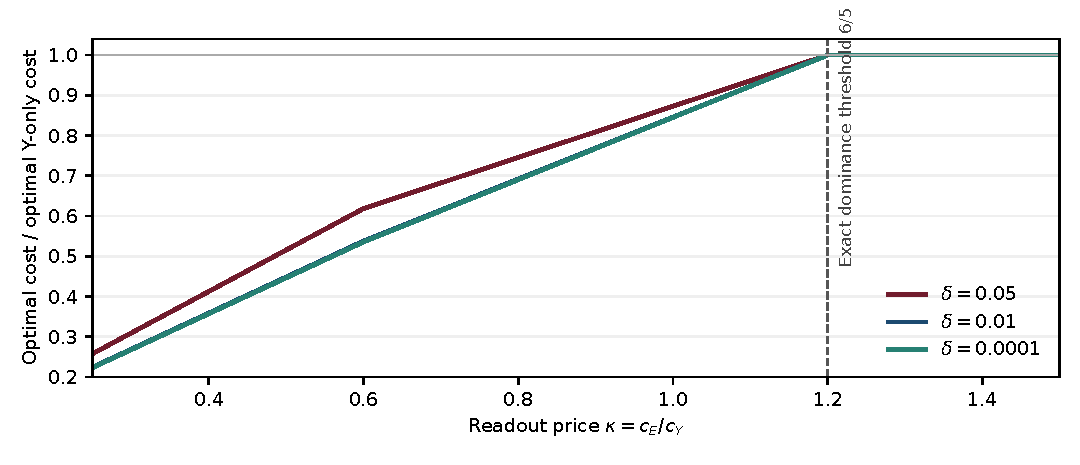
\includegraphics[width=.92\linewidth]{sharp_price_frontier.pdf}
 \caption{The exact confidence--price frontier of
 Theorem~\ref{thm:exact-price-frontier}, divided by the optimal $Y$-only
 cost. Every plotted price is checked by an exact rational primal--dual
 certificate. Lines join those samples; the equality plateau for
 $\kappa\geq6/5$ is proved for all prices, not inferred from the plot.
 The comparison concerns the two declared quantum readouts.}
 \label{fig:sharp-price-frontier}
\end{figure}

\paragraph{What is established and what is new in this development.}
The LP/Bellman method and controlled measurement selection have prior
theory \citep{fauss2015,lisensor2019}; the comparison-of-experiments principle
is classical \citep{blackwell1953}. The developments established here are
the explicit horizon-to-minimax bounds for the stated catalogue, the
parity-based exact confidence--price frontier, and its exactly realized
$6/5$ transition with rational optimality certificates. These supply a sharp, reproducible
characterization inside a declared model. They do not establish a new
general computational-complexity separation or priority over all work on
sequential experimental design.


\subsection{What the extension establishes}
The phase theorem remains a closed-form result for a restricted model.
The occupation and Bellman statements apply to finite-dimensional,
priced observation catalogues; the memory theorem permits collective
measurements inside blocks of growing size. These results make explicit
which arguments use qubit geometry, reflection symmetry, calibration,
or memory restrictions. They do not establish unrestricted quantum
computational speedups or solve arbitrary composite state families.
Composite sequential quantum testing already has separate asymptotic
theory \citep{simpson2026}; the band-calibration corollary above gives
a specific robust finite-cost guarantee rather than claiming that theory
as new. The exact lattice frontier optimizes every finite confidence and positive
readout price within its two-action family. Its quantum realizability
condition, the convergent catalogue programs, and the phase resource law
provide distinct levels of characterization; none silently enlarges the
admissible experiment class of another.
